%%%%%%%%%%%%%%%%%%%%%%%%%%%%%%%%%%%

% !TEX root = /home/eb/.vscode/qftrules.prepaworkshop/tmp/Exercice.tex
\begin{exo}[1][colle]{Théorie de Descartes de l'arc-en-ciel}
Une goutte d'eau sphérique d'indice de réfraction $n\simeq\SI{1.33}{}$ est éclairée par le Soleil. On suppose que l'air environnant est d'indice $n_{\rm air}\simeq1$. Soit $D_N$ la déviation angulaire totale d'un rayon pénétrant la goutte avec un angle d'incidence $i$ et ressortant de la goutte après $N$ réflexions internes partielles. $D_N$ est donc la différence entre l'angle d'entrée et l'angle de sortie.

\begin{center}
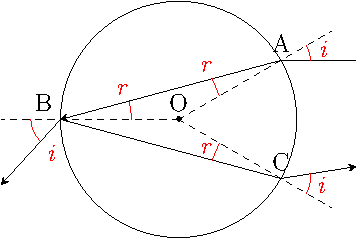
\includegraphics[scale=1]{goutte.pdf}
\end{center}

\begin{questions}
	\item À l'aide des lois de Snell-Descartes et de considérations géométriques simples, justifier que les angles d'incidence $i$ et de réfraction $r$ définis au point de rencontre du rayon incident avec la goutte, noté A, se retrouvent en B et C comme indiqué sur la figure. On ne demande pas de déterminer $r$ à ce stade.

	\solution{
		Les triangles $AOB$ et $AOC$ sont isocèles en $O$, et donc les angles opposés à $O$ sont égaux. On retrouve donc bien les angles $r$ comme indiqué sur le schéma.
	}
	\item Montrer qu'un rayon qui subit une réflexion interne subit une déviation angulaire $D_1=\pi-2r+2(i-r)$.   Généraliser au cas d'un rayon qui subit $N$ réflexions internes.

	\solution{La déviation angulaire associée à chaque réflexion interne vaut $\pi-2r$, et celle associée à chaque réfraction vaut $i-r$. La déviation angulaire totale vaut donc bien 
	$$
	\boxed{D_N=2(i-r)+N(\pi-2r)}.
	$$
}

	\item En utilisant les lois de Snell-Descartes, donner une relation entre l'angle de réfraction $r$ et l'angle d'incidence~$i$. En déduire la dérivée de $r$ par rapport à $i$, notée $\frac{\mathrm{d} r}{\mathrm{d} i}$. Montrer ensuite que
	$$
	\frac{\mathrm{d} D_1}{\mathrm{d} i} = 2-\frac{4}{n} \frac{\cos i}{\cos r}.
	$$

	\solution{On trouve
$$\frac{\mathrm{d} r}{\mathrm{d} i} = 	 \frac{1}{n} \frac{\cos i}{\cos r}.$$
	}

	\item Montrer que $\frac{\mathrm{d} D_1}{\mathrm{d} i}$ s’annule lorsque
	$$
	\sin^2(i) = \frac{4-n^2}{3}.
	$$
	En déduire que les rayons lumineux se concentrent autour d’une direction bien précise par rapport à la position du Soleil. Comment expliquer que les couleurs soient séparées dans un arc-en-ciel ?
	\solution{dispersion}

\end{questions}
\end{exo}
%%%%%%%%%%%%%%%%%%%%%%%%%%%%%%%%%%%%%%%%%%%%%%%%%%%%%%%%%%%%
